\chapter{Datasets}
\label{chap:datasets} 

In this chapter I introduce the datasets annotated using the tool described in chapter-\ref{chap:design}, describe a little background around each one and examine some statistics. It is left to chapter-\ref{chap:annotation} to  analyse the annotation process used to create these datasets and evaluate the annotation process.



\section{Size distributions}

\begin{figure}[ht]
\centering
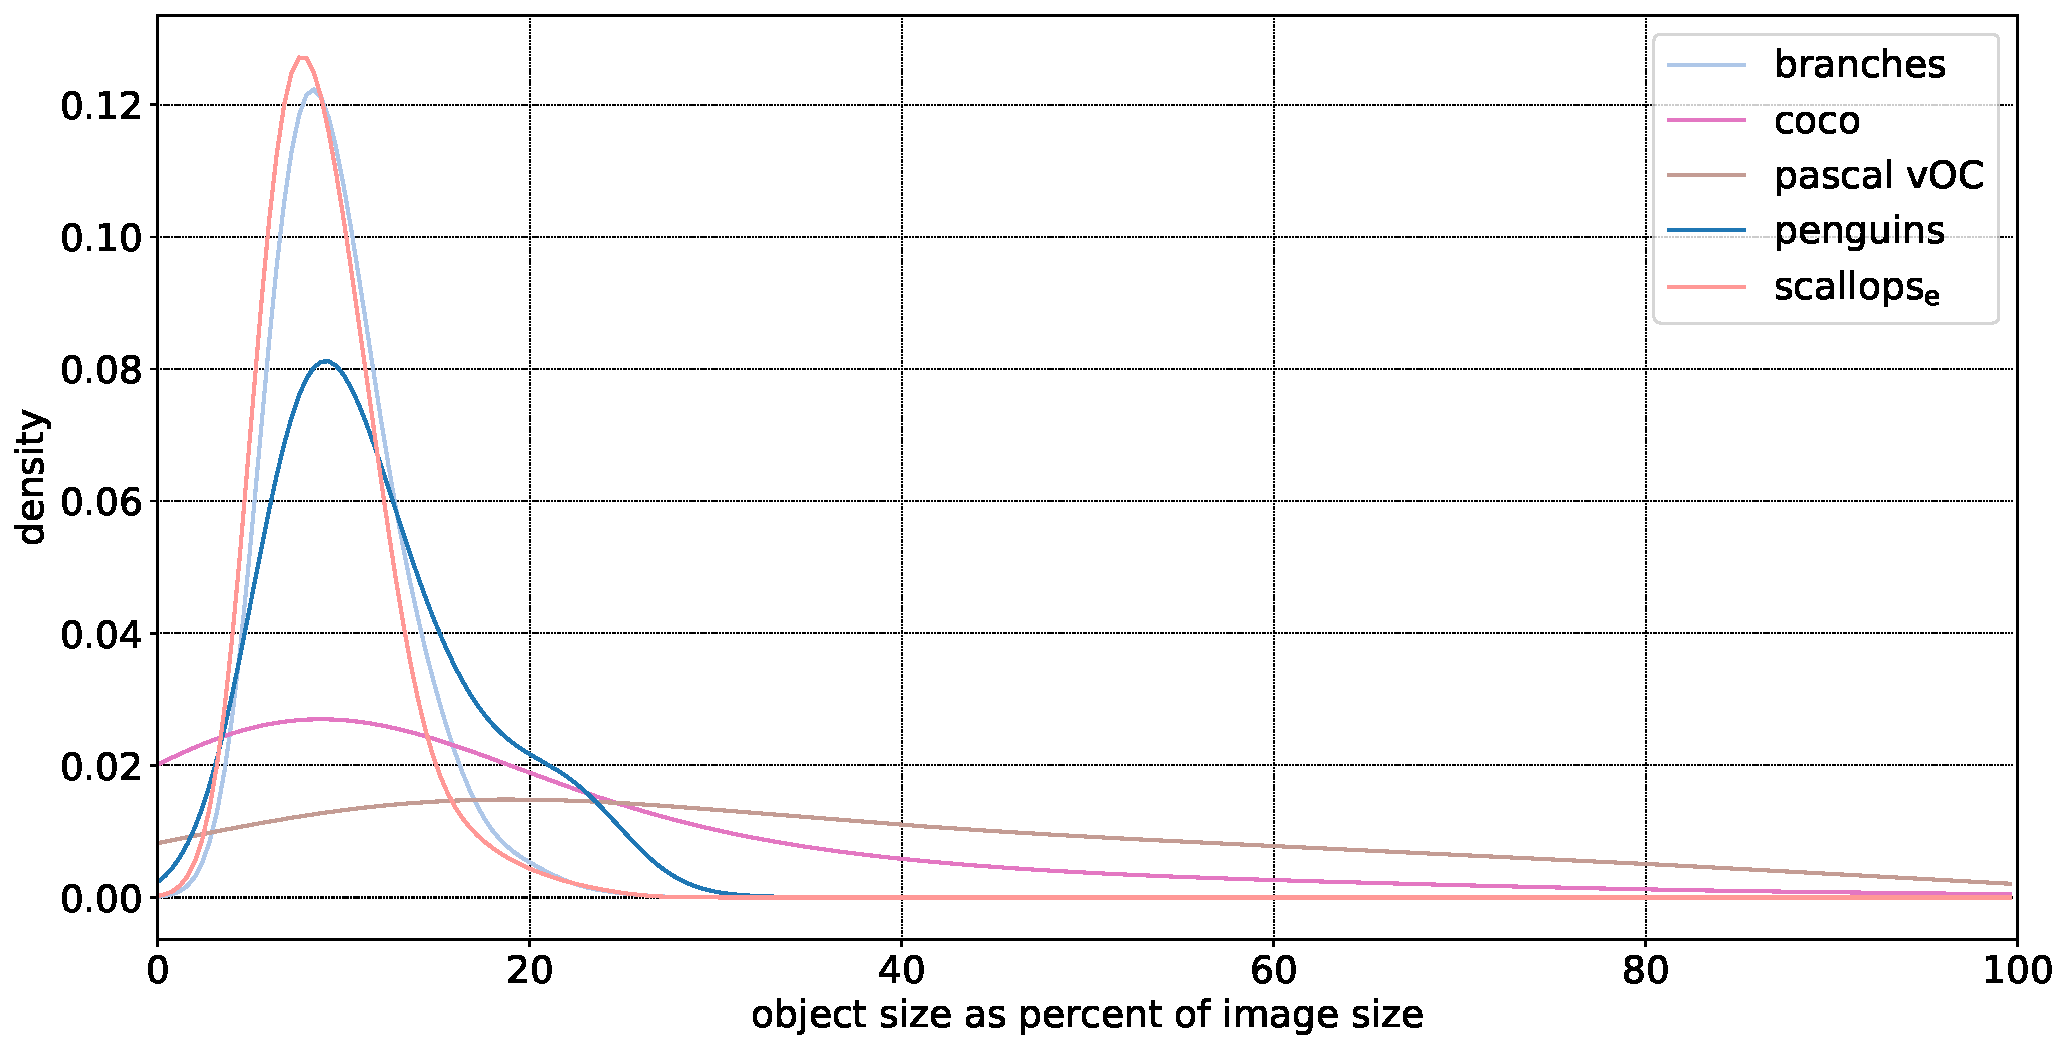
\includegraphics[width=0.9\linewidth]{charts/summaries/sizes_density.pdf}
\caption{Object bounding box size distributions as percent object to image size (average of width and height ratios) }
\label{fig:box_sizes}
\end{figure}







\begin{figure*}[h!]
\centering
\begin{subfigure}[t]{1.0\linewidth}
  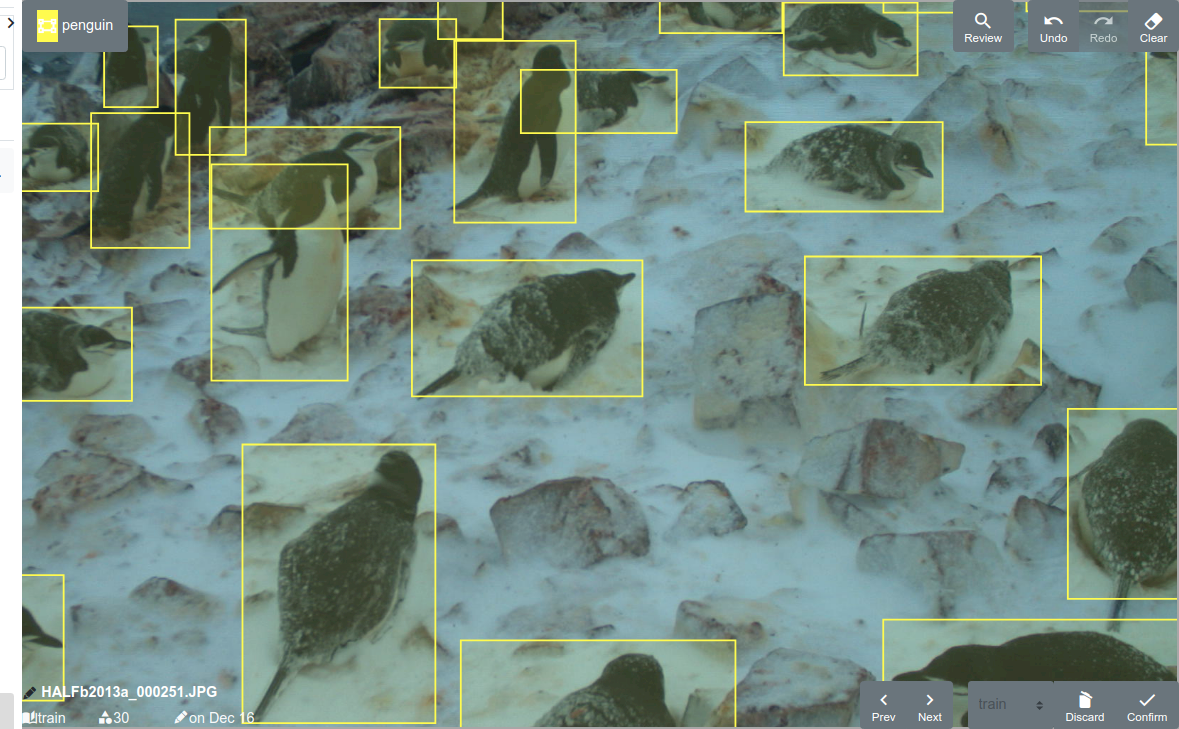
\includegraphics[width=0.475\linewidth]{figures/annotation/screenshots/penguins.png}
  \hfill
  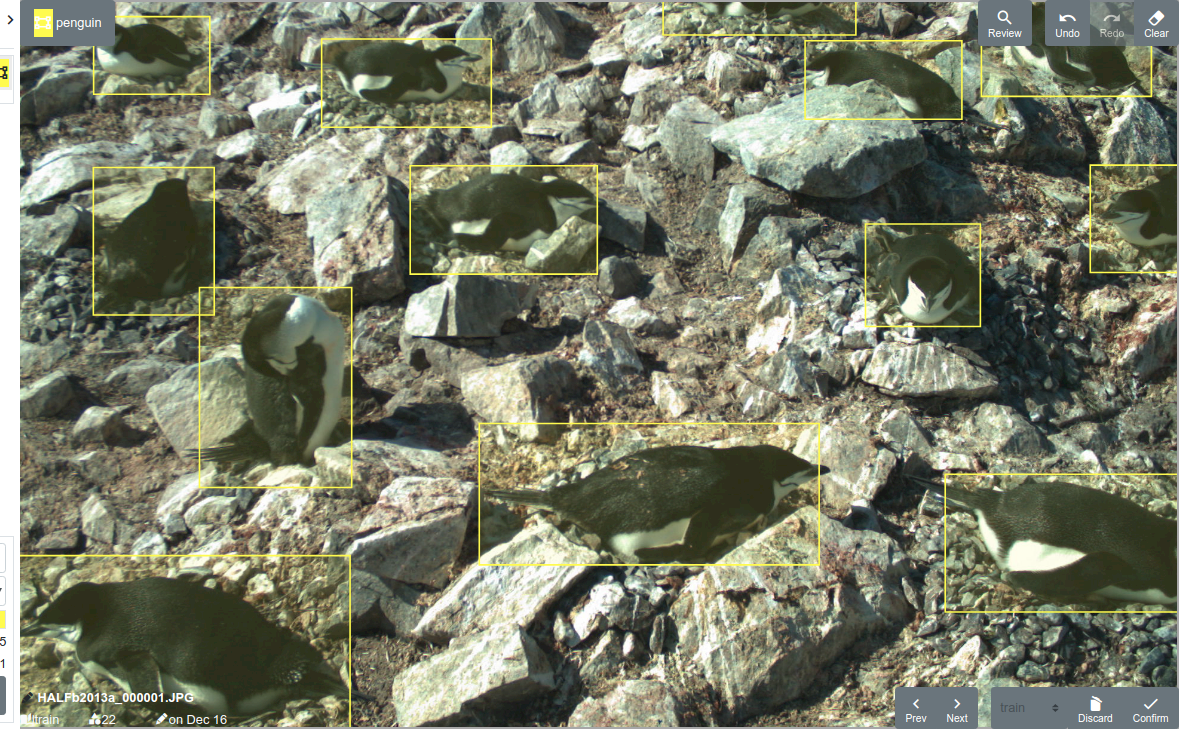
\includegraphics[width=0.475\linewidth]{figures/annotation/screenshots/penguins2.png}
  \caption{}
\end{subfigure}

\begin{subfigure}[t]{1.0\linewidth}
  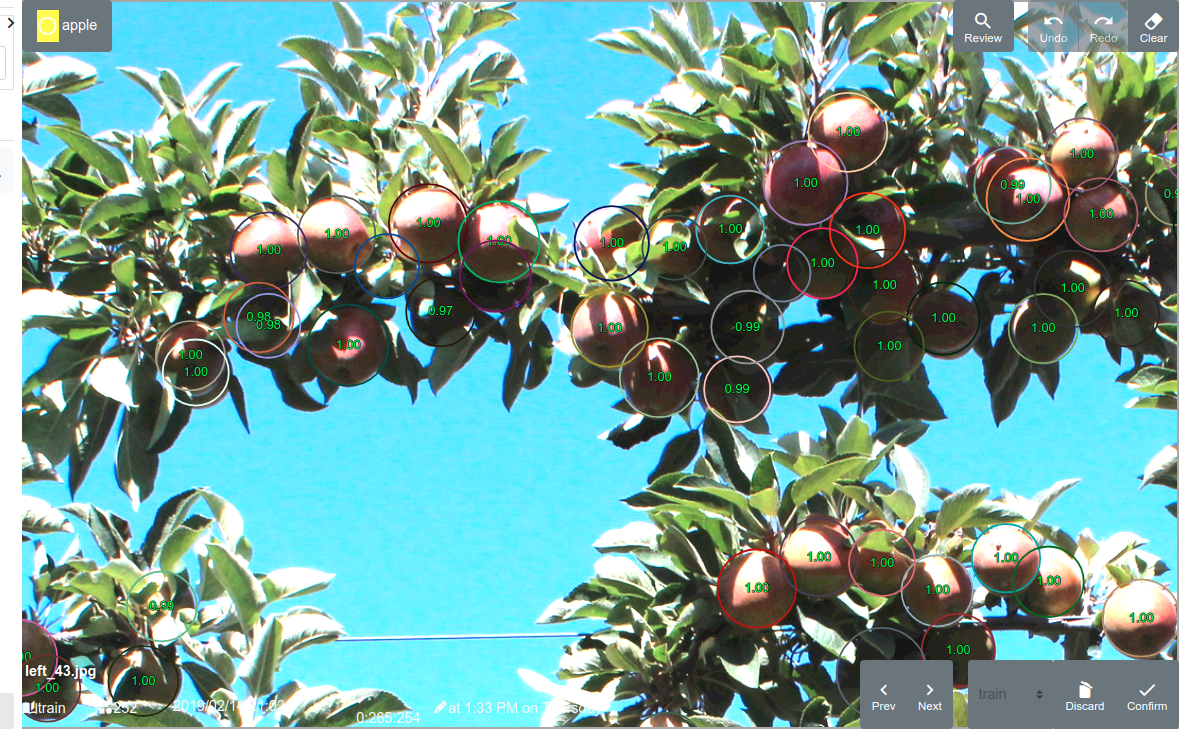
\includegraphics[width=0.475\linewidth]{figures/annotation/screenshots/apples_big.png}
  \hfill
  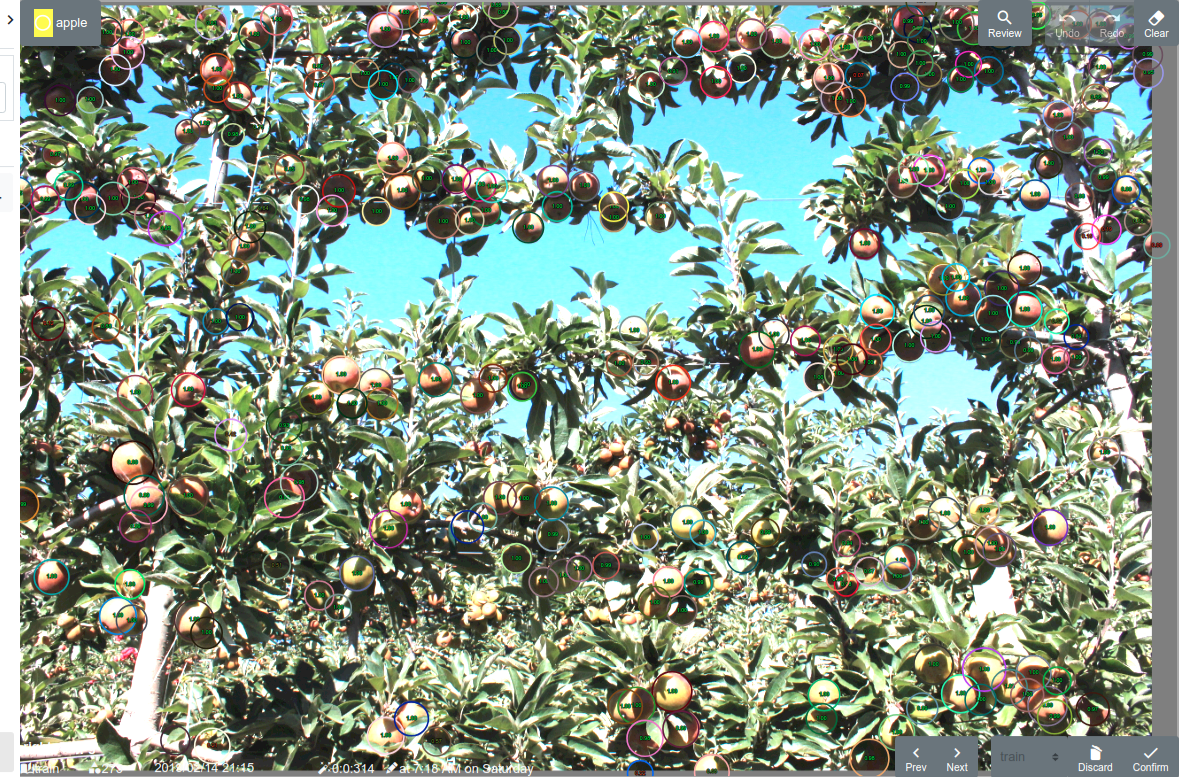
\includegraphics[width=0.475\linewidth]{figures/annotation/screenshots/apples_small.png}
  \caption{}
\end{subfigure}


\begin{subfigure}[t]{1.0\linewidth}
  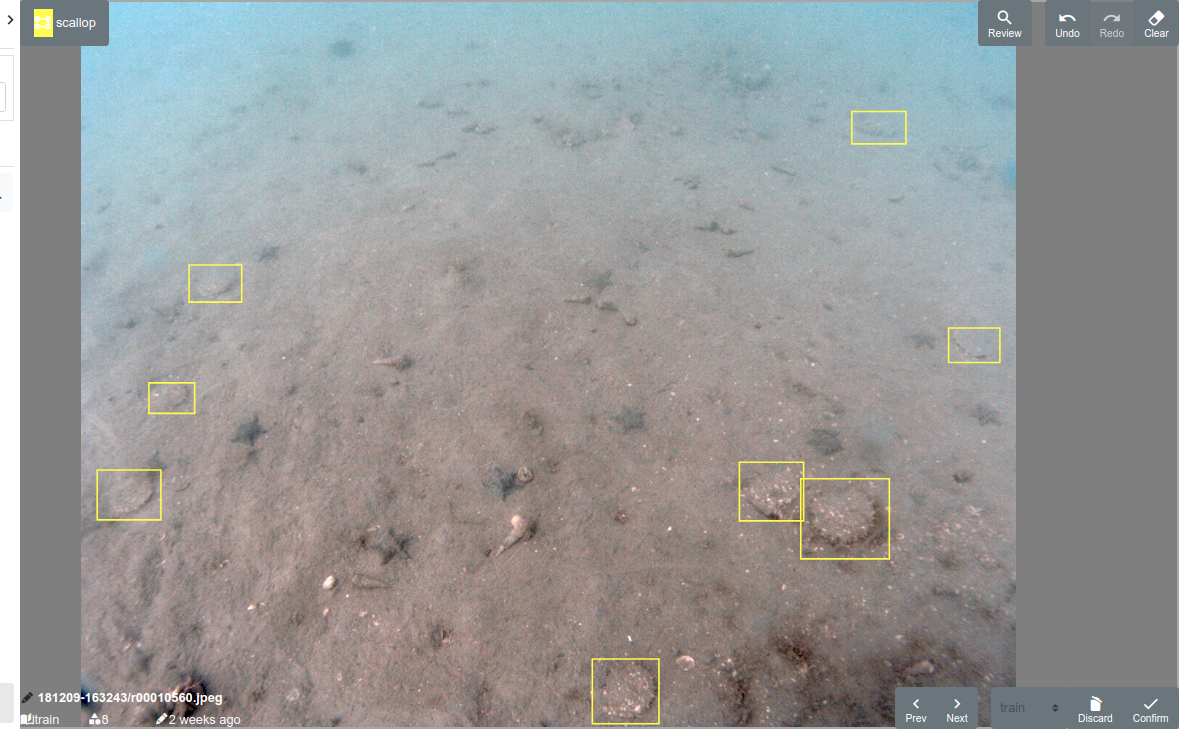
\includegraphics[width=0.475\linewidth]{figures/annotation/screenshots/scallops.png}
  \hfill
  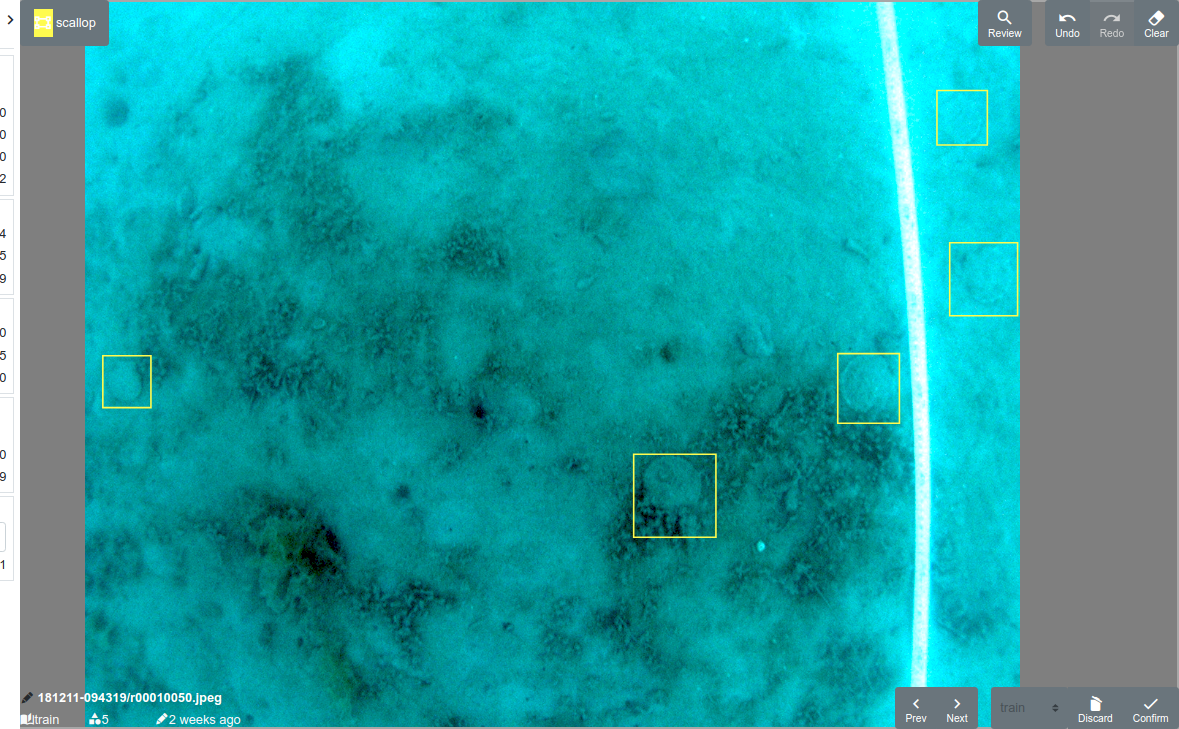
\includegraphics[width=0.475\linewidth]{figures/annotation/screenshots/scallops3.png}
  \caption{}

\end{subfigure}

\caption{ }
\label {fig:apple_examples}
\end{figure*}






\begin{figure*}[h!]
\centering

\begin{subfigure}[t]{0.5\textwidth}
  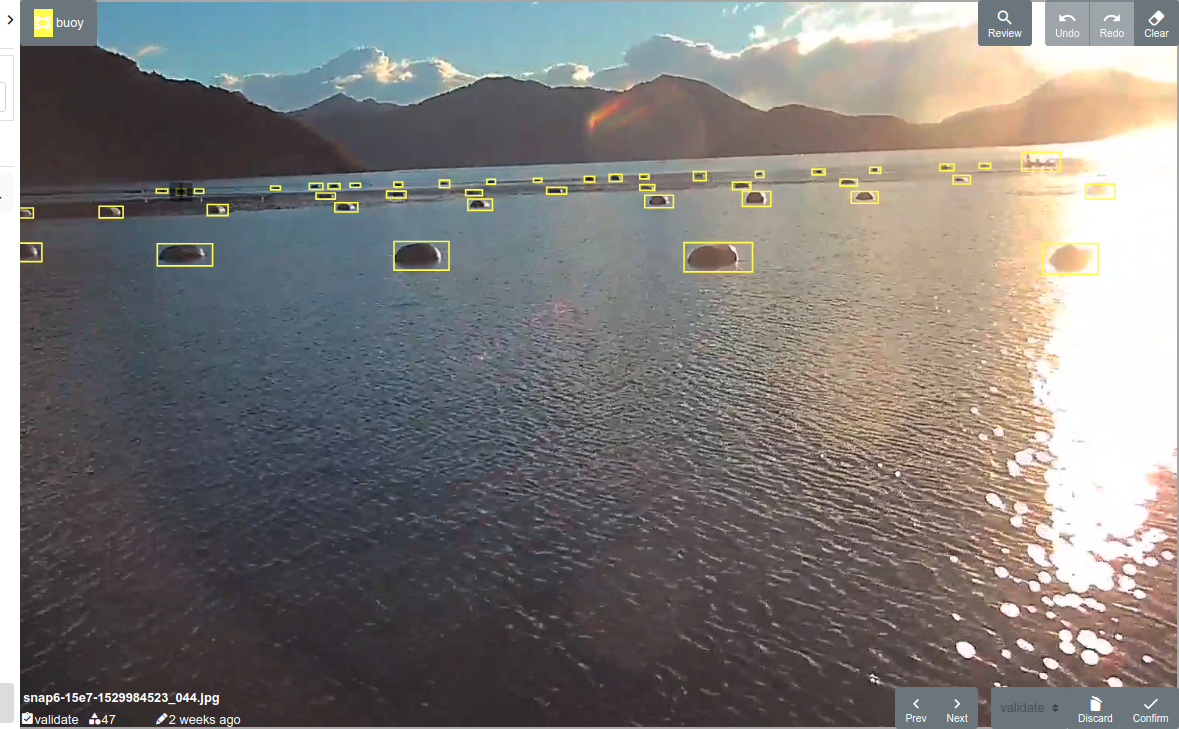
\includegraphics[width=0.95\textwidth]{figures/annotation/screenshots/buoys.png}
  \caption{}
\end{subfigure}%
\begin{subfigure}[t]{0.5\textwidth}
  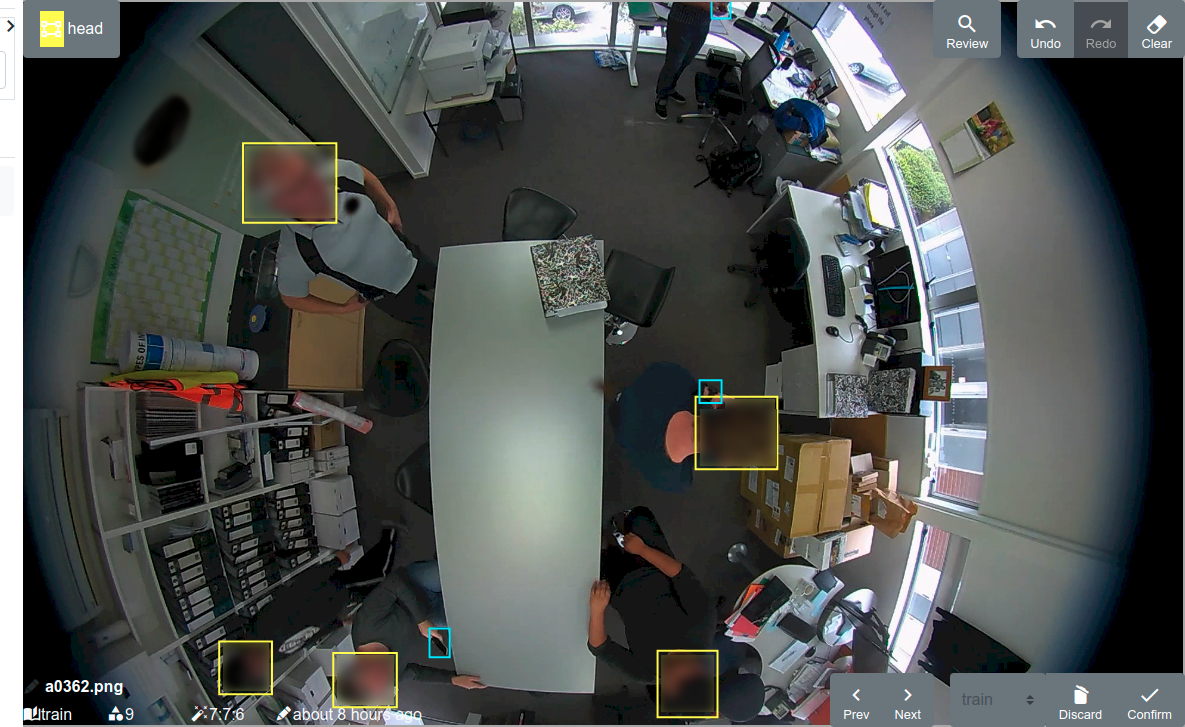
\includegraphics[width=0.95\textwidth]{figures/annotation/screenshots/victor.png}
  \caption{fisheye: Fish-eye head and cellphone detection }
\end{subfigure}

\begin{subfigure}[t]{0.5\textwidth}
  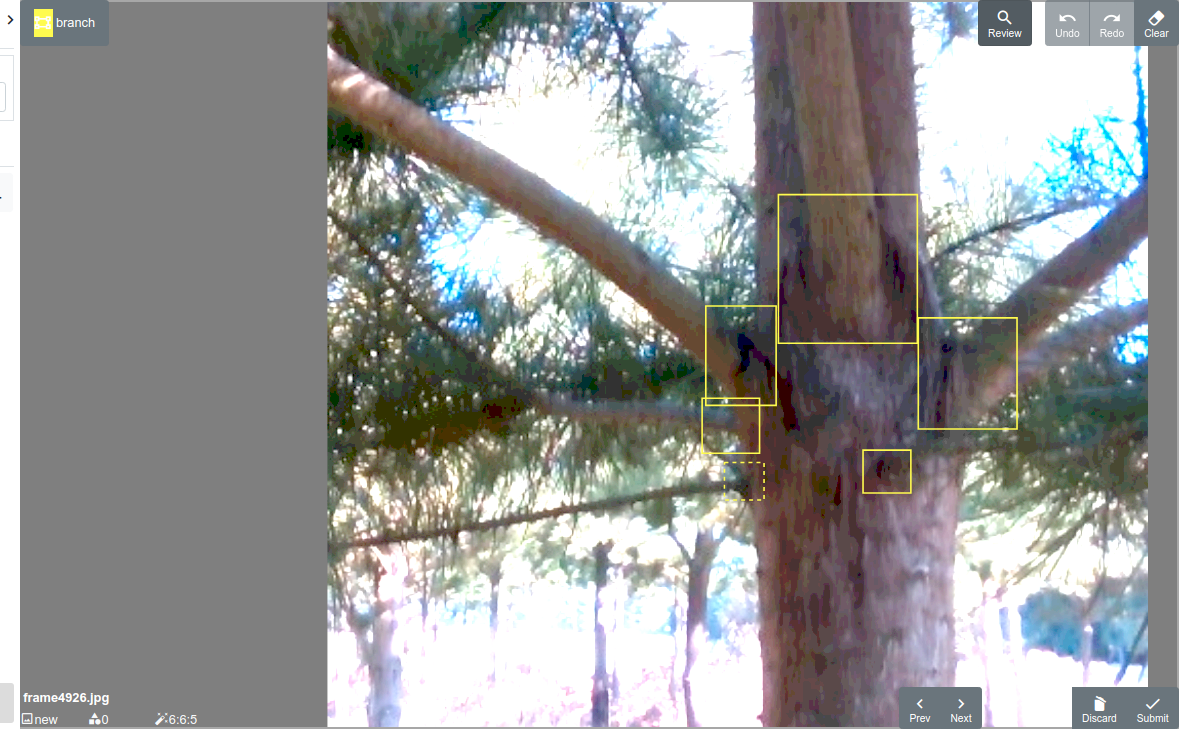
\includegraphics[width=0.95\textwidth]{figures/annotation/screenshots/branches3.png}
  \caption{branches: Tree branch intersection detection}
\end{subfigure}%
\begin{subfigure}[t]{0.5\textwidth}
  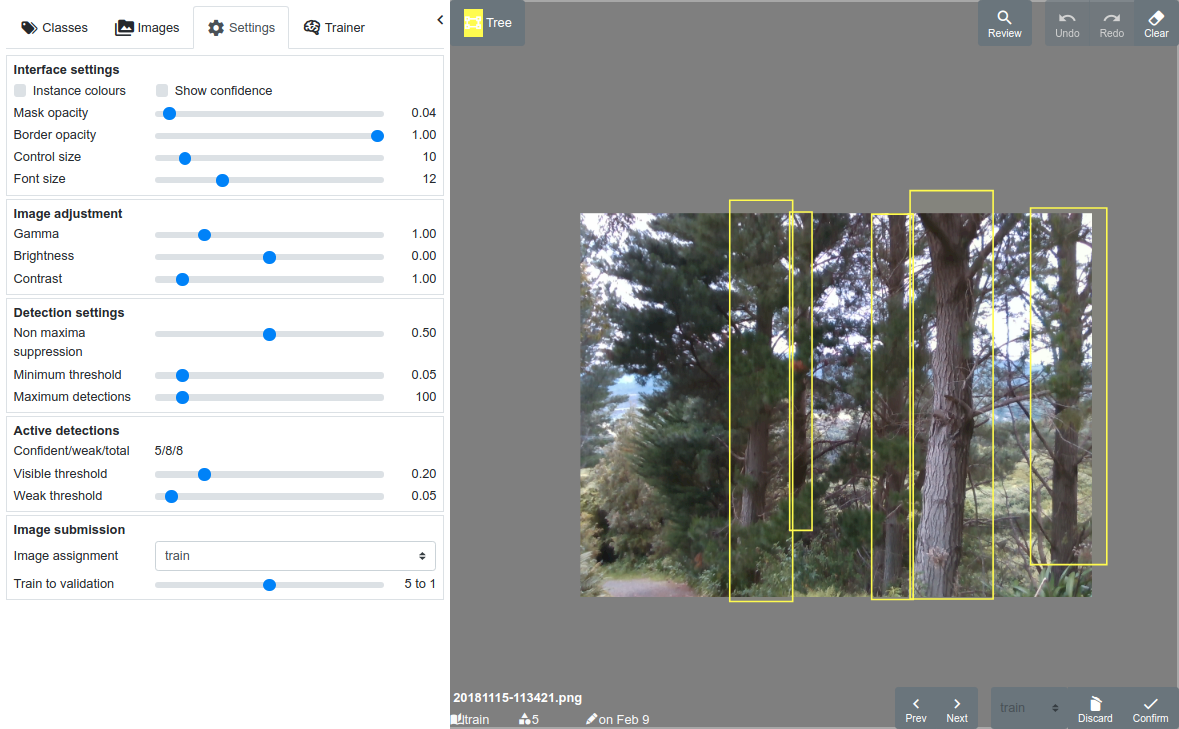
\includegraphics[width=0.95\textwidth]{figures/annotation/screenshots/josh_trees.png}
  \caption{}
\end{subfigure}

\caption{ }
\label {fig:dataset_images}
\end{figure*}